%! TEX root = lecture/Complex_Analysis

\subsection{The Riemann Zeta Function}
We proved in homework that the Riemann zeta function 
\begin{equation}
    \zeta(s)=\sum_{n=1}^\infty\frac{1}{n^s},\,s=\sigma+it
\end{equation}
is analytic in the half-plane  $ \Re s>1 $.
\begin{theorem}
    $ \zeta  $ has the following properties:
    \begin{enumerate}[label=(\alph*)]
        \item (Euler product formula)  $ \zeta  $ has the infinite product representation   \[\zeta(s)=\dps\prod_{p \text{ prime}}\frac{1}{1-p^{-s}},\, \Re s>1 \]
        \item  $ \zeta  $ extends to a meromorphic function on  $ \Cbb $ whose only poly is a simple pole at  $ s=1 $  with residue  $ 1 $.
        \item  $ \zeta  $ has no zeros in  $ \Re s \geq 1 $, all zeros of  $ \zeta $ in  $ \Re s \leq 0 $ are at  $ s=-2k $,  $ k\in \Nbb $. 
        \item  $ \zeta(2n)=\dps\frac{(-1)^{n-1}(2\pi )^{2n}}{2\cdot(2n)!}B_{2n} $,  $ n\in \Nbb $ where  $ B_{n} $ are the Bernoulli numbers, defined by  \[\dps\frac{z}{e^z-1}=\sum_{m=0}^\infty\frac{B_m}{m!}z^m ,\,|z|<2\pi \] 
        and  $ \zeta(-n)=-\dps\frac{B_{n+1}}{n+1},\,n\in \Nbb $.
        \item  $ \zeta  $ satisfies the functional equation  $ \zeta^*(1-s)=\zeta^*(s) $ where  $ \zeta^*  $ is the \name{symmetrized zeta function} defined by 
        \begin{equation}\label{eq:5.4:symmetrized zeta function}
            \zeta^*(s)=\pi^{-\frac{-\zeta}{2}}\Gamma(\frac{s}{2})\zeta(s)
        \end{equation}
        \item  $ \zeta^*(s)=\dps-\frac{1}{1-s}-\frac{1}{s}+\frac{1}{2}\int_1^\infty (t^{-\frac{s+1}{2}}+t^{\frac{s-2}{2}})(\theta(t)-1)\dd t $,  $ s\in \Cbb\setminus\{0,1\} $, where  $ \theta  $ is one of the \name{Jacobi theta series}, defined as 
        \begin{equation}\label{eq:5.4:Jacobi theta series}
            \theta(t)=\sum_{n=-\infty}^\infty e^{-\pi n^2t}
        \end{equation}
        \item  $ \zeta(s)=\dps\frac{\Gamma(1-s)}{2\pi i}\int_C\frac{(-z)^s}{e^z-1}\cdot\frac{\dd z}{z} $ where  $ C  $ is the contour shown in the picture, with  $ \epsilon<2\pi $,  $ (-z)^s=\exp[s\ln (-z)] $,  $ \ln(-z) $ is chosen \st  $ -\pi <\Im \ln (-z)<\pi $.        
        

        \tikzset{every picture/.style={line width=0.75pt}} %set default line width to 0.75pt        

        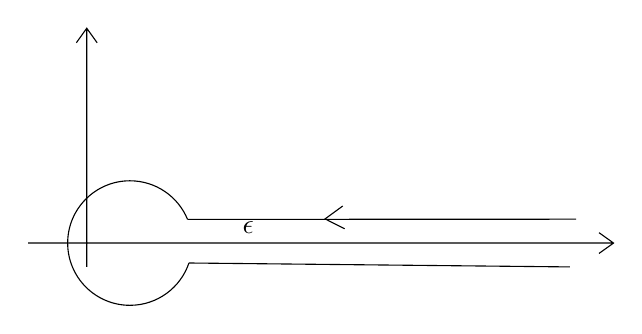
\begin{tikzpicture}[x=0.75pt,y=0.75pt,yscale=-1,xscale=1]
        %uncomment if require: \path (0,300); %set diagram left start at 0, and has height of 300

        %Shape: Axis 2D [id:dp9785911867399795] 
        \draw  (200,168.5) -- (482,168.5)(228.2,65) -- (228.2,180) (475,163.5) -- (482,168.5) -- (475,173.5) (223.2,72) -- (228.2,65) -- (233.2,72)  ;
        %Shape: Arc [id:dp1302548314750347] 
        \draw  [draw opacity=0] (277.43,178.11) .. controls (273.42,189.96) and (262.21,198.5) .. (249,198.5) .. controls (232.43,198.5) and (219,185.07) .. (219,168.5) .. controls (219,151.93) and (232.43,138.5) .. (249,138.5) .. controls (261.53,138.5) and (272.27,146.18) .. (276.76,157.1) -- (249,168.5) -- cycle ; \draw   (277.43,178.11) .. controls (273.42,189.96) and (262.21,198.5) .. (249,198.5) .. controls (232.43,198.5) and (219,185.07) .. (219,168.5) .. controls (219,151.93) and (232.43,138.5) .. (249,138.5) .. controls (261.53,138.5) and (272.27,146.18) .. (276.76,157.1) ;  
        %Straight Lines [id:da7349516742118151] 
        \draw    (276.76,157.1) -- (464,157) ;
        %Straight Lines [id:da49149077320950185] 
        \draw    (277.43,178.11) -- (461,180) ;
        \draw   (351.53,150.65) -- (343.02,156.87) -- (352.44,161.61) ;

        % Text Node
        \draw (302,157) node [anchor=north west][inner sep=0.75pt]   [align=left] {$\displaystyle \epsilon $};


        \end{tikzpicture}

    \end{enumerate}
\end{theorem} 
\begin{proof}
    (a)  $ \dps\prod_{p\text{ prime}}\frac{1}{1-p^{-s}}=\frac{1}{\dps \prod_{p\text{ primes}}(1-p^{-s})} $,  $ \Re s>1 $ converges absolutely since  $ \dps\sum_{p\text{ prime}}|p^{-s}|=\sum_{p\text{ prime}}p^{-\Re s} $ converges for  $ \Re s>1 $. Hence,  $ F(s)=\dps\prod_{p\text{ prime}}\frac{1}{1-p^{-s}} $.     
\end{proof}